% Falta uma introdução do capítulo!


In other countries and locations there have been initiatives for creating the so-called nanogrids, in which an optimized peer-to-peer topology \cite{MAGNASCO2016369} can be obtained by specialized real time management devices.
In this sense, we could expect an ever more active transactive energy.



% Detalhar mais que o texto descrito no Apêndice, porém buscar identificar conceito de sistema e não da engenharia elétrica

The \glsreset{gd}\gls{gd} is an alternative power source to the traditional big power plants.
At Brazil, the former comprises mainly photovoltaic solar panels to feed local power demands, while the latter encompass hydroeletric and thermoelectric power plants to sustain the country power needs.

% Diferença entre micro e mini
The \gls{gd} has its limits based on power capacity installations, i.e., at the Brazilian context, if the \gls{gd} installation has up to 75 kW of power capacity it is considered a micro grid, however if greater than this and up to 5 MW it is considered a mini grid.
Note that it is independently of the source type and must be connected to the local power distribution grid~\cite{GD}.
% completar com a diferença para o tamanho do SIN
% For the sake of comparison, the \gls{sin} has ... GW of power capacity.
As a matter of curiosity, the \gls{sin} has about 162 GW of power capacity~\cite{BIG2}.

Whilst the benefits of electricity to the daily life of society is immeasurable, the cost to do so is controversial.
The Brazilian policy aims to support the captive consumers%
\footnote{For a better comprehension about captive and free consumers consider \autoref{appen:1}.}
with the lowest possible tariff, and with a tariff diversification based on different energy scenarios in the country.
However, those that profit with \gls{gd} installation have an additional option of power source and electricity tariff to choose from.
No matter the reasons, if it is greener or a look for energy independence, the \gls{gd} offers an alternative to feed distinctive power needs.

Therefore, the captive consumers%
\footnote{An explanation about captive consumers is also at \autoref{appen:1}.}
can now be classified beyond their power consumption levels
with those that produce electricity being known as \emph{prosumers} (\emph{pro}ducer + con\emph{sumer}).
The prosumers are grouped by the Brazilian regulation into four categories,
but they can be divided into two main groups based on their generation management,
one that is for self-consumption, and another for shareable consumption.
The former is for individual use.
The \gls{gd} may be on the same local of power consumption or
in another place -- namely \emph{remote self-consumption} -- whereas the power and consumption units must be inside the same distribution utility coverage area.
The latter refers to sharing generation between customers,
either they are from a condominium -- known as \emph{enterprises of multiple consumer units} -- or
from a consortium or a cooperative -- known as a \emph{shareable generation}.
Again, the customers' units must situate inside the same distribution utility coverage area.
\autoref{fig:gd-categories} summarizes this classification and contextualizes the \gls{gd} into the power energy sector.

\begin{figure}[h!tbp]{\textwidth}
    \centering
    \caption{Classification of \gls{gd} under the Brazilian legislation, and its positioning in the power sector chain.}
    \label{fig:gd-categories}
    
    \tikzstyle{arrow} = [thick, ->, >=stealth, line width=1pt]
    \tikzstyle{drew} = [draw, fill=white, rounded corners=0.1cm, align=center]
    \tikzstyle{powers} = [align=center]
    
    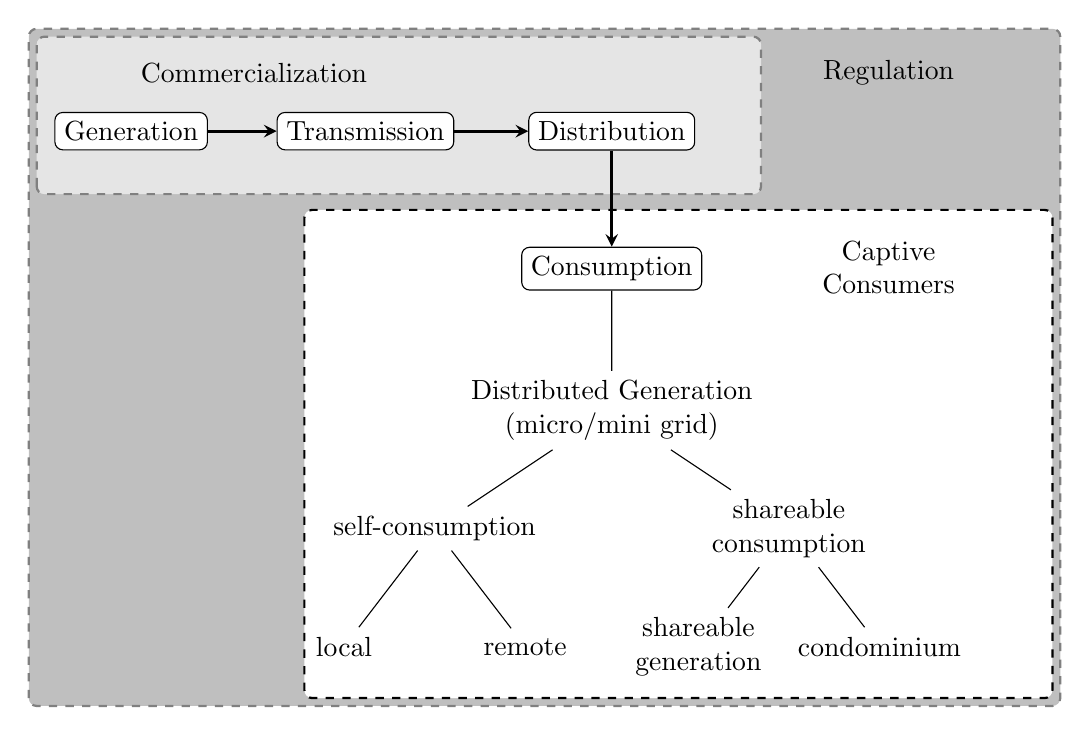
\begin{tikzpicture}[level 1/.style={powers,level distance=1.8cm},%
                        level 2/.style={powers, level distance=1.5cm, sibling distance=4.5cm},%
                        level 3/.style={powers, level distance=1.5cm, sibling distance=2.3cm}]
        % place dimensions
        \draw[gray, thick, dashed, fill=gray!50, rounded corners=0.1cm] (-2,-7.3) rectangle (11.1,1.3);
        \draw[drew, thick, dashed] (1.5,-1) rectangle (11,-7.2);
        \draw[gray, thick, dashed, fill=gray!20, rounded corners=0.1cm] (-1.9,-0.8) rectangle (7.3,1.2);
        
        % place nodes
        \node[drew] at (-0.7,0)             (g) {Generation};
        \path (g.east)+(2,0) node[drew]     (t) {Transmission};
        \path (t.east)+(2,0) node[drew]     (d) {Distribution};
		\path (d.south)+(0,-1.5) node[drew] (c) {Consumption}
		    child { node {Distributed Generation\\(micro/mini grid)}
		        child { node {self-consumption}
		            child { node {local} }
		            child { node {remote} }
		        }
		        child { node {shareable\\consumption}
    		        child { node {shareable\\generation} }
    		        child { node {condominium} }
    		    }
	        };
        \path (g.north)+(0,0.5)	node[anchor=west] (o) {Commercialization};
        \path (o.east)+(6.5,0) node               (r) {Regulation};
        \path (r.south)+(0,-2.2) node[align=center] {Captive\\Consumers};

        % draw connections
        \draw[arrow] (g) -- (t);
        \draw[arrow] (t) -- (d);
        \draw[arrow] (d) -- (c);
        
    \end{tikzpicture}
    
%   	\legend{Although the \gls{gd} is a tiny portion of the whole sector, it has a huge impact on the captive consumers.}
    \source{Author.}
\end{figure}

% Como a distribuição de energia acontece na GD?
Even with different categories, the delivery of electricity follows the same principle to distribute the total power generation ($E_{T}$) by the number of participants over their own agreement.
\autoref{eq:power distribution} catches this behaviour with the number of participants ($n$) ranging from 1, as the individual case, to multiple members ($m$), as the shareable case.

\begin{equation}\label{eq:power distribution}
    E_{T} = \sum_{n=1}^{m} E_{n} \qquad \text{[Wh]}
\end{equation}

Specific exceptions guide how the cost and benefit of an investment in the \gls{gd} will be split among the participants.
For instance, the remote self-consumption case has more than one participant to share electricity, but only one person responsible to sustain the related investment.
On the other hand, for the condominium case, multiple people are taken into account.
Thus, the attribution of cost and benefit is determined by each category guidelines.
However, one common sharing operation is to distribute energy proportionally to each member investment contribution,
i.e., an investment of 10\% guarantees 10\% of the electricity generated in a given period.
This model represents the investment shares as percentage values, called as well as quotas.

So, \autoref{eq:quotas} complements the \autoref{eq:power distribution} arranging the dual relationship of cost and benefit for a particular person.
Consequently, the electricity obtained by a member ($E_{m}$) can be interpreted as a weighted value ($q_{m}$) of the \gls{gd} cost ($C_{DG}$), i.e., of the total power generation ($E_{T}$).

\begin{equation}\label{eq:quotas}
    E_{m} = q_{m} \cdot C_{DG} \qquad \text{[Wh]}
\end{equation}

% Como acontece a distribuição de créditos?
Nonetheless, independently of group type,
the surplus energy generated can be ``stored'' on the distribution grid by no additional cost%
\footnote{Until the expected approval of changes on the \href{http://www.aneel.gov.br/audiencias-publicas?p_auth=pWIuCaW3&p_p_id=audienciaspublicasvisualizacao_WAR_AudienciasConsultasPortletportlet&p_p_lifecycle=1&p_p_state=normal&p_p_mode=view&p_p_col_id=column-2&p_p_col_count=1&_audienciaspublicasvisualizacao_WAR_AudienciasConsultasPortletportlet_audienciaId=2301&_audienciaspublicasvisualizacao_WAR_AudienciasConsultasPortletportlet_javax.portlet.action=visualizarAudiencia}{\emph{Resolução Normativa n\textsuperscript{o} 482/2012}} in the year of 2019.}
in order to be consumed later, a measure known in Brazil as the Electricity Compensation System~\cite{FAQ}. % [ANEEL, 2016a]
However, this ``energy credit'' can only be used for personal purposes, i.e., it can not be transferred for anyone, even if part of a shareable consumption group.
The surplus energy depends on each member consumption rate over her/his power quota.

In general, the power generated must be known by the distribution utility in order to keep record of the energy credit that will be distributed.
But beyond to what is exposed by \autoref{eq:power distribution}, the utility must get notes about member's quotas as well, because each member has a personal consumer profile, and consequently, a different energy credit balance.
\autoref{fig:ecredits} depicts how this management between the generation and the credit is handled.
For the cases of the shareable consumption group, the generation is accountable as a unit and later distributed proportionally by each member's quota.

% (angle:distance) :: -360º <= angle <= 720º

\def\upperarrow{
            (sg.north east)+(-0.5,0) arc (0:130:3.8) [rounded corners=0.5]
                -- +(0:0.25) [rounded corners=0.5]
                -- +(-109:0.662) [sharp corners]
                -- +(180:0.65) [rounded corners=0.5]
                -- +(180:0.42) [rounded corners=0.5]
                -- +(180:0.42) arc (132:0:4.3) [rounded corners=0.5]
                -- cycle
              }
              
\def\bottomarrow{
            (d.south west)+(0.5,-0.1) arc (-45:0:-3) [rounded corners=0.5]
                % início seta 1
                -- +(-45:0) arc (0:105:-1) [rounded corners=0.5]
                -- +(100:0.15) [rounded corners=0.5]
                -- +(15:0.4) [sharp corners]
                -- +(-70:0.3) [rounded corners=0.5]
                -- +(-70:0.2) [sharp corners]
                -- +(-70:0.2) arc (115:30:-1.1) [sharp corners]
                % fim seta 1
                -- +(0:0) arc (30:90:-1.5) [rounded corners=0.5]
                % início seta 2
                -- +(0:0) arc (91:109:-7.5) [rounded corners=0.5]
                -- +(100:0.15) [rounded corners=0.5]
                -- +(15:0.4) [sharp corners]
                -- +(-70:0.3) [rounded corners=0.5]
                -- +(-70:0.2) [sharp corners]
                -- +(-70:0.2) arc (109:102:-8.5) [sharp corners]
                % fim seta 2
                % início seta 3
                -- +(0:0) arc (90:110:-10.5) [rounded corners=0.5]
                -- +(100:0.15) [rounded corners=0.5]
                -- +(15:0.4) [sharp corners]
                -- +(-70:0.3) [rounded corners=0.5]
                -- +(-70:0.2) [sharp corners]
                -- +(-70:0.2) arc (115:110:-11.5) [sharp corners]
                % fim seta 3
                % início seta 4
                -- +(0:0) arc (95:108:-11) [rounded corners=0.5]
                -- +(100:0.15) [rounded corners=0.5]
                -- +(15:0.4) [sharp corners]
                -- +(-70:0.3) [rounded corners=0.5]
                -- +(-70:0.2) [sharp corners]
                -- +(-70:0.2) arc (110:90:-12.5) [sharp corners]
                % fim seta 4
                -- +(0:0) arc (90:83:-18.5) [rounded corners=0.5]
                -- +(0:0) arc (83:55:-3) [rounded corners=0.5]
                -- +(0,0) arc (47:35:-2.5) [rounded corners=0.5]
                -- +(0,0) arc (30:-45:-2.5) [rounded corners=0.5]
                -- cycle
            }

\begin{figure}[h!t]{\textwidth}
	\centering
    \caption{definir...} \label{fig:ecredits}
    
    \tikzstyle{arrow} = [thick,->,>=stealth, line width=1pt]
    \tikzstyle{drew} = [draw,fill=white,rounded corners=0.1cm]
    
    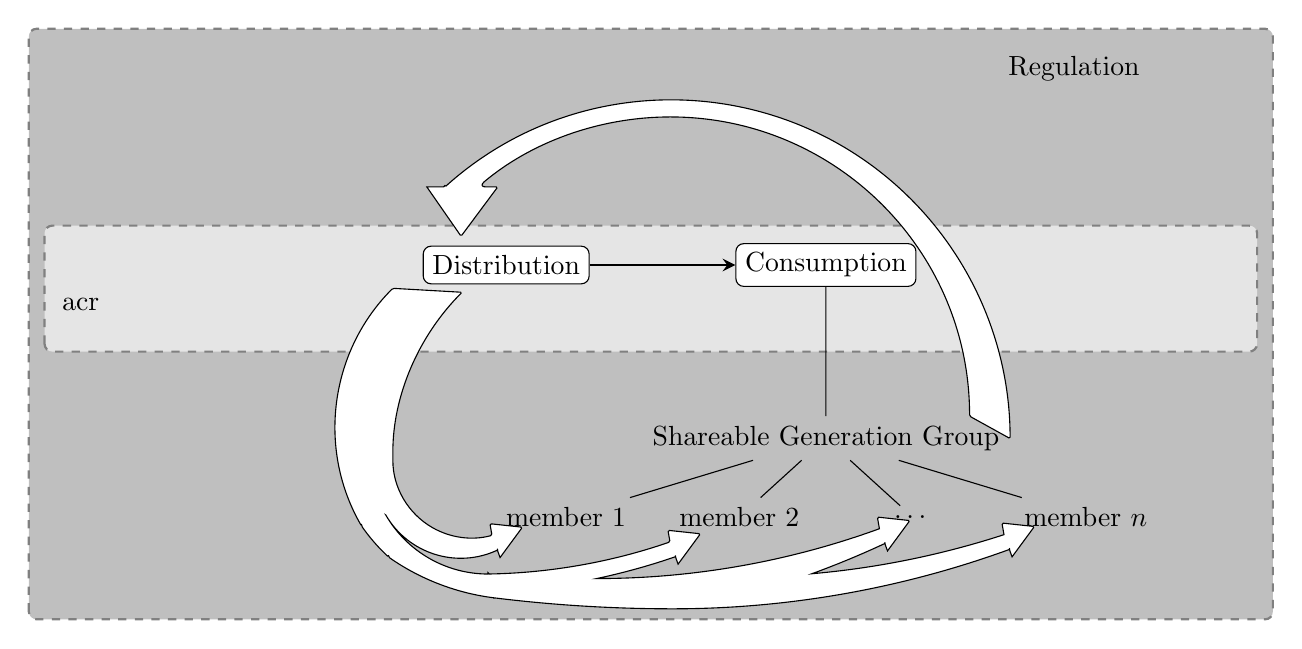
\begin{tikzpicture}[level 1/.style={level distance=2.2cm}, level 2/.style={level distance=1cm, sibling distance=2.2cm}]
        % place dimensions
        \draw[gray,thick,dashed,fill=gray!50,rounded corners=0.1cm] (-2,-6) rectangle (13.8,1.5);
        \draw[gray,thick,dashed,fill=gray!20,rounded corners=0.1cm] (-1.8,-2.6) rectangle (13.6,-1);
        
        % place nodes
        \node[anchor=west, text width=10em]	at (-1.7, -2)	(o) {\gls{acr}};
        \path (o.east)+(2,0.5) node[drew] (d) {Distribution};
		\path (d.east)+(3,0) node[drew] (c) {Consumption}
		    child { node (sg) {Shareable Generation Group}
		        child { node (m1) {member 1} }
		        child { node {member 2} }
		        child { node {\dots} }
		        child { node {member $n$} }
	       % \foreach \k in {1,...,10}{
	       %     child { node {member \k} }
	       % } % dá errado 
	        };
        \path (c.east)+(2,2.5) node		(r) {Regulation};
        
        % draw connections
        \draw[arrow] (d) -- (c);
        \draw[drew] \upperarrow;
        \draw[drew] \bottomarrow;
        
    \end{tikzpicture}
    
  	\legend{\textcolor{red}{AINDA ESTÁ ERRADO!} Differences between energy credit distribution among dwellers of a \gls{gd} group.}
    \source{Author.}
\end{figure}

% Physical System Operation and Planning |x| Market Operation